% =====================================================================
% Fleven - Slides tecnicos
% Compile no Overleaf (ou texlive completo) com pdfLaTeX:
%   pdflatex -> bibtex -> pdflatex -> pdflatex
% Requer: beamer (tema metropolis), pgfplots, tikz, booktabs.
% Se o tema "metropolis" nao estiver disponivel, troque a linha
%   \usetheme{metropolis}  ->  \usetheme{Madrid}   (tema embutido)
% =====================================================================
\documentclass[aspectratio=169,11pt]{beamer}

\usetheme{metropolis}

\usepackage[utf8]{inputenc}
\usepackage[T1]{fontenc}
\usepackage[brazil]{babel}
\usepackage{amsmath, amssymb}
\usepackage{booktabs}
\usepackage{tikz}
\usepackage{pgfplots}
\pgfplotsset{compat=1.18}
\usetikzlibrary{positioning, arrows.meta}

% ---- Paleta da marca Fleven ----
\definecolor{flamber}{HTML}{F5970A}
\definecolor{fldark}{HTML}{0A0A0F}
\definecolor{flblue}{HTML}{2563EB}
\definecolor{flgreen}{HTML}{22C55E}
\definecolor{florange}{HTML}{C2410C}

\setbeamercolor{frametitle}{bg=fldark, fg=flamber}
\setbeamercolor{progress bar}{fg=flamber, bg=flamber!30}
\setbeamercolor{title separator}{fg=flamber}
\setbeamercolor{alerted text}{fg=florange}
\metroset{block=fill}

\setbeamertemplate{bibliography item}{}

\title{Fleven}
\subtitle{Federated Learning for Vehicular Environments}
\author{João C. Braz \and José Wilson C. Souza \and Erick de Souza Lima \and Mina Monteiro}
\institute{LAINF}
\date{\today}

\begin{document}

% ---- Capa com o logo do Fleven como herói e o Inmetro como afiliação ----
\begin{frame}[plain]
  \centering
  \vspace{1.0cm}
  
\includegraphics[width=0.58\textwidth]{figures/logo-fleven.png}

  {\Large Federated Learning for Vehicular Environments\par}

  \vspace{.3cm}
  {\small João C. Braz \quad José Wilson C. Souza \quad Erick de Souza Lima \quad Mina Monteiro\par}
  \vspace{0.25cm}

  \vfill
  
\includegraphics[height=1.25cm]{figures/logo-inmetro.png}
  \vspace{0.4cm}
\end{frame}

\section{Aprendizado Federado}

\begin{frame}{A ideia do Aprendizado Federado}
  \begin{columns}[T]
    \begin{column}{0.5\textwidth}
      Apenas os pesos aprendidos do modelo.
      \medskip

      O ciclo, a cada \emph{round}:
      \begin{enumerate}
        \item O servidor distribui o modelo global $\theta_g$.
        \item Cada cliente treina com seus próprios dados.
        \item Cada cliente devolve seus pesos $\theta_k$.
        \item O servidor agrega os pesos em um novo modelo global.
      \end{enumerate}
      \medskip

    \end{column}
    \begin{column}{0.5\textwidth}
      \centering
      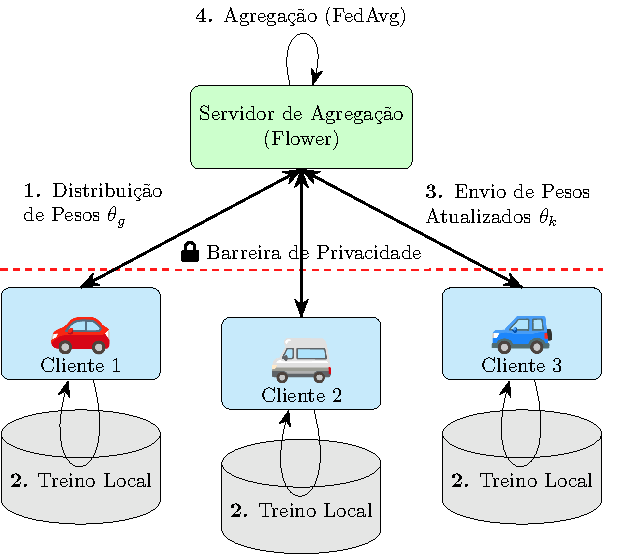
\includegraphics[width=\linewidth]{figures/fl_arquiteture.pdf}
    \end{column}
  \end{columns}
\end{frame}

% =====================================================================
\section{Estratégias de Agregação}

\begin{frame}{Como uma rede neural aprende}
  \begin{columns}[T]
    \begin{column}{0.54\textwidth}
      Uma rede neural é uma função com muitos \textbf{pesos} nas conexões. O conjunto
      de todos os pesos é o $\theta$.
      \medskip

      \textbf{Aprender} = ajustar $\theta$ para reduzir o \emph{erro} entre a previsão
      e o valor real:
      \[
        \theta \;\leftarrow\; \theta \;-\; \eta\, \nabla_\theta \mathcal{L}
      \]
      {\footnotesize $\mathcal{L}$: erro (perda);\quad $\eta$: taxa de aprendizado;\\
       $\nabla_\theta \mathcal{L}$: direção que mais reduz o erro.}
      \medskip

      No Aprendizado Federado é esse $\theta$ que cada veículo aprende localmente
      e envia ao servidor.
    \end{column}
    \begin{column}{0.46\textwidth}
      \centering
      \begin{tikzpicture}[>=Stealth,
        nrn/.style={circle, draw=fldark!60, minimum size=6.5mm, inner sep=0},
        lbl/.style={font=\scriptsize}]
        \node[nrn, fill=flblue!25]  (I1) at (0,1.2)   {};
        \node[nrn, fill=flblue!25]  (I2) at (0,0)     {};
        \node[nrn, fill=flblue!25]  (I3) at (0,-1.2)  {};
        \node[nrn, fill=flamber!40] (H1) at (1.8,1.8) {};
        \node[nrn, fill=flamber!40] (H2) at (1.8,0.6) {};
        \node[nrn, fill=flamber!40] (H3) at (1.8,-0.6){};
        \node[nrn, fill=flamber!40] (H4) at (1.8,-1.8){};
        \node[nrn, fill=flgreen!40] (O1) at (3.6,0)   {};
        \foreach \i in {1,2,3}{\foreach \j in {1,2,3,4}{\draw[->, gray!45] (I\i) -- (H\j);}}
        \foreach \j in {1,2,3,4}{\draw[->, gray!45] (H\j) -- (O1);}
        \node[lbl] at (0,-2.5)   {entradas};
        \node[lbl] at (1.8,-2.6) {camadas ocultas};
        \node[lbl] at (3.6,-2.5) {previsão};
      \end{tikzpicture}
      \\[2pt]
      {\scriptsize Cada seta é um peso; o conjunto de pesos é o $\theta$.}
    \end{column}
  \end{columns}
\end{frame}

\begin{frame}{FedAvg}
  A estratégia base é a \textbf{média ponderada} pelos dados de cada cliente
  \cite{mcmahan2017communication}: clientes com mais amostras pesam mais.

  \[
    \theta_{t+1} \;=\; \sum_{k=1}^{K} \frac{n_k}{n}\, \theta_k^{\,t+1},
    \qquad n = \sum_{k=1}^{K} n_k
  \]

  \begin{itemize}
    \item $\theta_k^{\,t+1}$: pesos do cliente $k$ após o treino local.
    \item $n_k$: número de amostras do cliente $k$.
  \end{itemize}
  \medskip
  \begin{alertblock}{Experimentos}
    O FedAvg foi a estratégia \textbf{mais estável} nos grupos de veículos.
  \end{alertblock}
\end{frame}

\begin{frame}{Otimizadores adaptativos}
  As demais estratégias tratam a diferença dos pesos como um \alert{pseudo-gradiente}
  e aplicam um otimizador \emph{no servidor} \cite{reddi2021adaptive}:
  \[
    \Delta_t = \sum_{k} \tfrac{n_k}{n}\big(\theta_k^{t+1}-\theta_t\big),
    \qquad
    m_t = \beta_1 m_{t-1} + (1-\beta_1)\,\Delta_t
  \]
  \[
    \theta_{t+1} = \theta_t + \eta\,\frac{m_t}{\sqrt{v_t}+\tau}
  \]
  A diferença está em como cada um acumula a variância $v_t$:
  \begin{center}
  \small
  \begin{tabular}{ll}
    \toprule
    \textbf{Estratégia} & \textbf{Atualização de $v_t$} \\
    \midrule
    FedAdagrad & $v_t = v_{t-1} + \Delta_t^2$ \\
    FedAdam    & $v_t = \beta_2 v_{t-1} + (1-\beta_2)\,\Delta_t^2$ \\
    FedYogi    & $v_t = v_{t-1} - (1-\beta_2)\,\Delta_t^2\,\mathrm{sign}(v_{t-1}-\Delta_t^2)$ \\
    \bottomrule
  \end{tabular}
  \end{center}
\end{frame}

% =====================================================================
\section{FedPer: personalização}

\begin{frame}{FedPer}
  O FedPer  divide o modelo para conciliar
  \alert{conhecimento coletivo} e \alert{particularidades de cada veículo} \cite{arivazhagan2019fedper}.
  \begin{columns}[T]
    \begin{column}{0.5\textwidth}
      \textbf{\textcolor{flblue}{Cabeça global (LSTM)}}
      \begin{itemize}
        \item Compartilhada entre todos.
        \item Agregada pelo servidor (FedAvg).
        \item Aprende padrões temporais gerais.
      \end{itemize}
      \medskip
      \textbf{\textcolor{flgreen}{Cauda local (Dense)}}
      \begin{itemize}
        \item Específica de cada veículo.
        \item \textbf{Nunca} é enviada ao servidor.
        \item Aprende o comportamento individual.
      \end{itemize}
    \end{column}
    \begin{column}{0.5\textwidth}
      \centering
      \begin{tikzpicture}[node distance=6mm, font=\scriptsize]
        \node[draw, rounded corners, fill=flblue!20, minimum width=3.2cm, minimum height=8mm] (lstm) {Extrator temporal (LSTM) - global};
        \node[draw, rounded corners, fill=flgreen!20, below=of lstm, minimum width=3.2cm, minimum height=8mm] (dense) {Predição (Dense) - local};
        \node[below=4mm of dense] (out) {previsão de consumo};
        \draw[-{Stealth}] (lstm) -- (dense);
        \draw[-{Stealth}] (dense) -- (out);
        \node[right=2mm of lstm, text width=2.2cm, align=left] {\textcolor{flblue}{sobe ao servidor}};
        \node[right=2mm of dense, text width=2.2cm, align=left] {\textcolor{flgreen}{fica no veículo}};
      \end{tikzpicture}
    \end{column}
  \end{columns}
  \medskip
\end{frame}

% =====================================================================
\section{Modelagem temporal}

\begin{frame}{Janela deslizante}
  A série de leituras vira pares $(X, Y)$: $X$ é o \textbf{passado} usado como
  contexto e $Y$ é o \textbf{futuro} a prever. A janela desliza ponto a ponto.
  \begin{center}
  \begin{tikzpicture}[font=\footnotesize]
    % pontos da serie
    \foreach \i in {0,...,11} {
      \fill[fldark] (\i*0.72,0) circle (2.2pt);
      \node[below] at (\i*0.72,-0.15) {$t_{\i}$};
    }
    % janela X (contexto)
    \draw[flblue, thick, rounded corners]
      (-0.25,-0.55) rectangle (5.0,0.55);
    \node[flblue] at (2.4,0.85) {$X$: janela de entrada};
    % janela Y (previsao)
    \draw[flgreen, thick, rounded corners]
      (5.15,-0.55) rectangle (7.9,0.55);
    \node[flgreen] at (6.5,0.85) {$Y$: horizonte};
    % seta
    \draw[-{Stealth}, florange, thick] (2.4,-0.9) -- (6.5,-0.9);
    \node[florange, below] at (4.4,-0.95) {desliza (\texttt{stride})};
  \end{tikzpicture}
  \end{center}
  
\end{frame}

% =====================================================================
\section{Arquitetura: Flower}

\begin{frame}{Federação, SuperLink e SuperNode}
  O Fleven usa o \textbf{Flower} para orquestrar o treino.
  \begin{itemize}
    \item \textbf{Federação}: o conjunto servidor + clientes que treinam juntos,
          com suas regras de conexão.
    \item \textbf{SuperLink} (servidor): distribui o modelo, recebe os pesos e
          \textbf{agrega}. Roda em um ponto central.
    \item \textbf{SuperNode} (cliente): roda embarcado em cada veículo
          (ex.\ Raspberry Pi), treina localmente e devolve apenas os pesos.
  \end{itemize}
  \medskip
  \begin{center}
  \begin{tikzpicture}[font=\footnotesize, node distance=8mm]
    \node[draw, rounded corners, fill=flgreen!15] (link) {SuperLink (servidor)};
    \node[draw, rounded corners, fill=flblue!12, below left=10mm and 12mm of link] (n1) {SuperNode 1};
    \node[draw, rounded corners, fill=flblue!12, below=12mm of link] (n2) {SuperNode 2};
    \node[draw, rounded corners, fill=flblue!12, below right=10mm and 12mm of link] (n3) {SuperNode $N$};
    \draw[{Stealth}-{Stealth}] (link) -- (n1);
    \draw[{Stealth}-{Stealth}] (link) -- (n2);
    \draw[{Stealth}-{Stealth}] (link) -- (n3);
  \end{tikzpicture}
  \end{center}
\end{frame}

% =====================================================================
\section{Experimentos}

\begin{frame}{Dados}
  \begin{columns}[T]
    \begin{column}{0.54\textwidth}
      Base \textbf{eVED}: 184 veículos.
      \medskip

      Veículos agrupados por \textbf{motorização, cilindrada e peso}
      \medskip

      \textbf{Features} (entradas):
      \begin{itemize}
        \item Velocidade do veículo (km/h)
        \item MAF, fluxo de ar (g/s)
        \item Rotação do motor (RPM)
        \item Carga absoluta do motor (\%)
      \end{itemize}
      \textbf{Target}: consumo de energia (kWh).
    \end{column}
    \begin{column}{0.44\textwidth}
      \centering \small
      \begin{tabular}{lc}
        \toprule
        Grupo & Clientes \\
        \midrule
        G01 · HEV 1.8L   & 14 \\
        G02 · HEV 1.5L   & 13 \\
        G03 · ICE 2.4L   & 7  \\
        G04 · ICE 2.5L   & 7  \\
        G05 · ICE 2.0L   & 6  \\
        \bottomrule
      \end{tabular}
    \end{column}
  \end{columns}
\end{frame}

\begin{frame}{O target consumo de energia}
  É a energia (em kWh) consumida em cada leitura OBD ($\approx 1s$).
  \smallskip

  \textbf{Combustão (ICE) e híbridos (HEV)} - do fluxo de ar (MAF) e das correções
  de combustível (\emph{fuel trims}):
  \[
    EC = \frac{v}{3600 \cdot 100}\, \cdot\, MAF \,\cdot\, 3{,}785 \,\cdot\,
         \frac{1 + \frac{STFT}{100} + \frac{LTFT}{100}}{AFR \cdot 0{,}1123}
  \]

  \textbf{Plug-in (PHEV) e elétricos (EV)} - direto da bateria de alta tensão:
  \[
    EC = -\,\frac{I_{HV} \cdot V_{HV}}{3{,}6 \times 10^{6}}
  \]

  \smallskip
  {\footnotesize
  \textbf{onde:}\;
  $v$: velocidade (km/h);\quad
  $MAF$: fluxo de ar (g/s);\quad
  $STFT,\,LTFT$: correções de curto e longo prazo da mistura ar-combustível (\%);\quad
  $AFR = 14{,}08$: razão ar-combustível da gasolina;\quad
  $I_{HV},\,V_{HV}$: corrente (A) e tensão (V) da bateria de alta tensão.
  As constantes fazem as conversões de unidade ($1\,\text{kWh} \approx 0{,}1123\,\text{L}$ de gasolina).}
\end{frame}

\begin{frame}{Configurações testadas}
  \begin{columns}[T]
    \begin{column}{0.5\textwidth}
      \textbf{Modelos}
      \begin{itemize}
        \item LSTM
        \item LSTM + Dense
        \item MLP
        \item \textbf{FedPer} (personalizado)
      \end{itemize}
      \medskip
      \textbf{Estratégias de agregação}
      \begin{itemize}
        \item FedAvg, FedAdam
        \item FedYogi, FedAdagrad
      \end{itemize}
    \end{column}
    \begin{column}{0.5\textwidth}
      \textbf{Principais hiperparâmetros}
      \centering \small
      \begin{tabular}{ll}
        \toprule
        Parâmetro & Valor \\
        \midrule
        Janela de entrada    & 50 leituras \\
        Horizonte            & 5 leituras \\
        Rounds federados     & 20 \\
        Épocas locais/round  & 3 \\
        Camada oculta (LSTM) & 64 \\
        Taxa de aprendizado  & $10^{-3}$ \\
        \bottomrule
      \end{tabular}
    \end{column}
  \end{columns}
  \vspace{4pt}
  \footnotesize \emph{grupo × modelo × estratégia} foi executada e
  registrada para comparação.
\end{frame}

\begin{frame}{Análise exploratória dos dados}
  Antes de treinar, analisemos o target e o volume de dados por cliente (grupo G01).
  \begin{columns}[T]
    \begin{column}{0.5\textwidth}
      \centering
      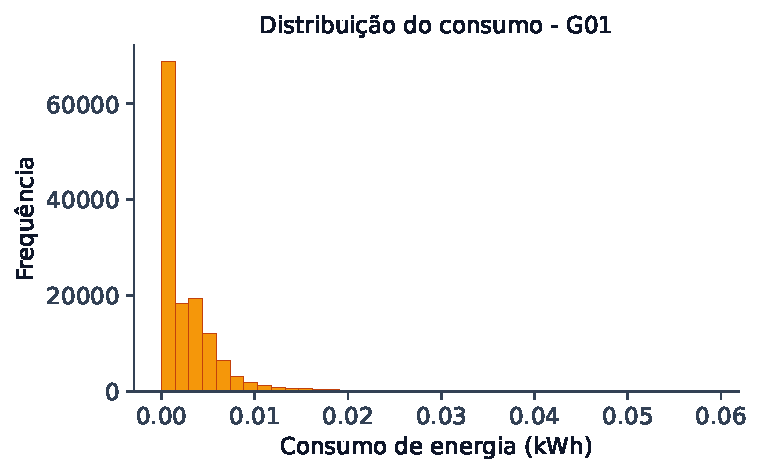
\includegraphics[width=\linewidth]{figures/eda_target_dist.pdf}
      \\ {\scriptsize muitos valores baixos, cauda longa.}
    \end{column}
    \begin{column}{0.5\textwidth}
      \centering
      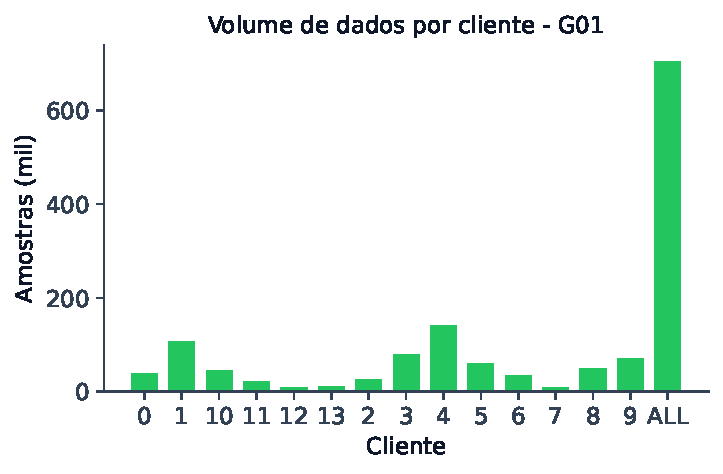
\includegraphics[width=\linewidth]{figures/eda_samples.pdf}
      \\ {\scriptsize O volume de dados varia bastante entre os veículos.}
    \end{column}
  \end{columns}
  \vspace{2pt}
  \footnotesize A heterogeneidade entre clientes  motiva o uso de personalização.
\end{frame}

\begin{frame}{Análise exploratória: features}
  \begin{columns}[T]
    \begin{column}{0.53\textwidth}
      \centering
      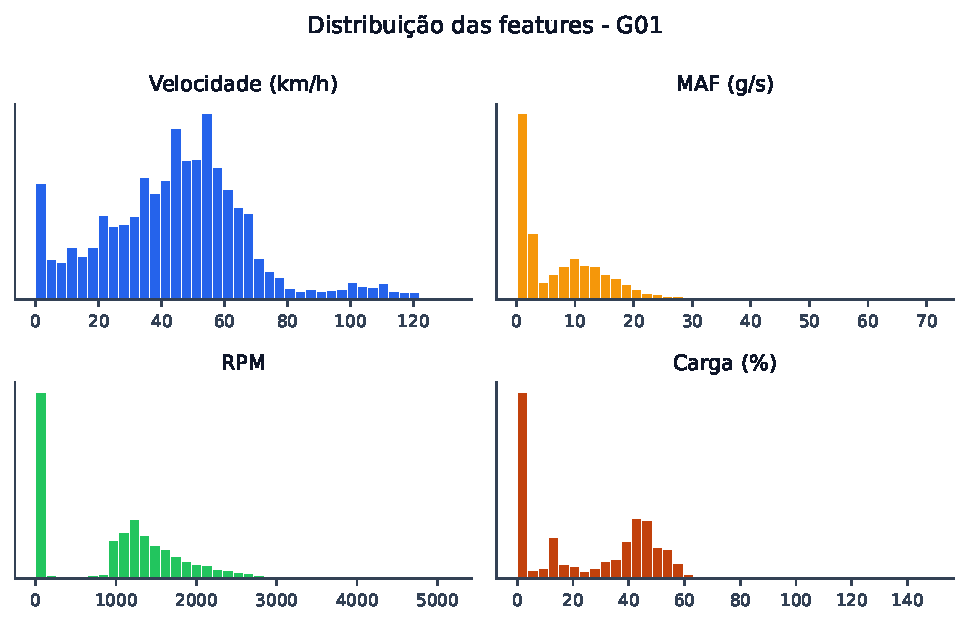
\includegraphics[width=\linewidth]{figures/eda_features.pdf}
    \end{column}
    \begin{column}{0.45\textwidth}
      \centering
      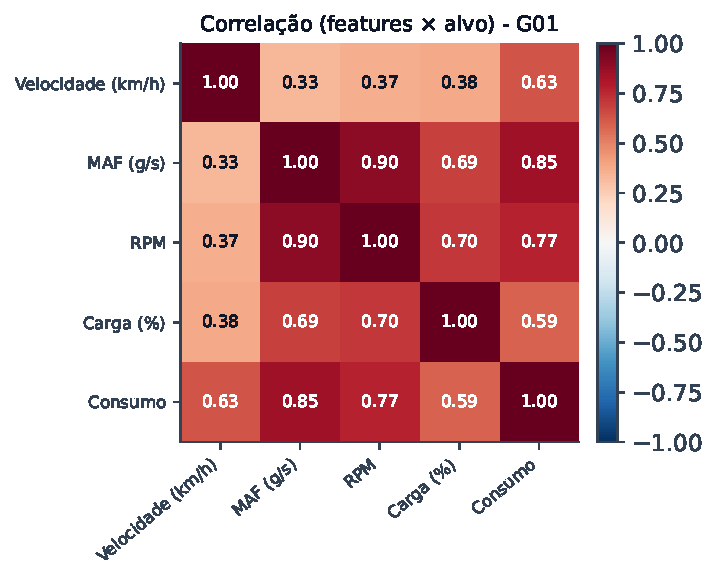
\includegraphics[width=0.98\linewidth]{figures/eda_corr.pdf}
    \end{column}
  \end{columns}
  \vspace{2pt}
  \footnotesize O \textbf{MAF} (fluxo de ar) é a variável mais correlacionada com o
  consumo ($0{,}85$), seguida da rotação (RPM); velocidade e carga contribuem de
  forma complementar. Faz sentido físico: o consumo é derivado do fluxo de ar.
\end{frame}

\begin{frame}{Convergência: curvas de perda (G01)}
  \begin{columns}[T]
    \begin{column}{0.5\textwidth}
      \centering
      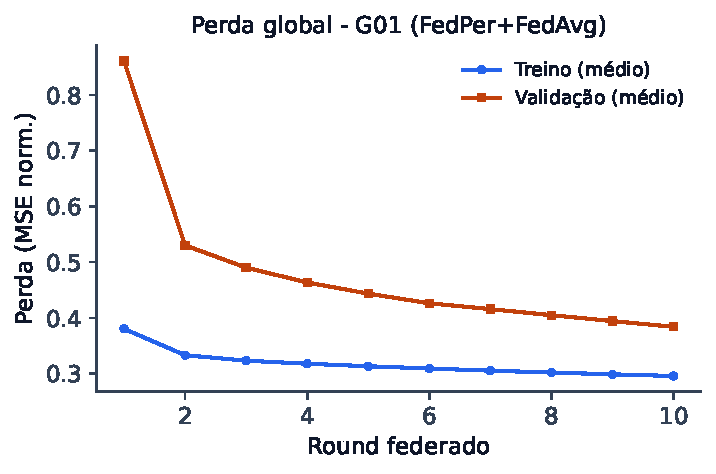
\includegraphics[width=\linewidth]{figures/loss_global.pdf}
      \\ {\scriptsize A perda média (treino e validação) cai e estabiliza ao longo dos rounds.}
    \end{column}
    \begin{column}{0.5\textwidth}
      \centering
      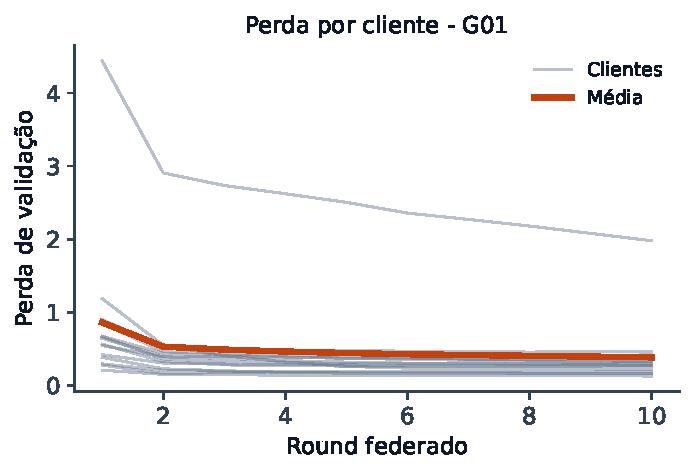
\includegraphics[width=\linewidth]{figures/loss_per_client.pdf}
      \\ {\scriptsize Cada cliente converge; um veículo com sensor ausente fica acima.}
    \end{column}
  \end{columns}
  \vspace{2pt}
  \footnotesize A perda é medida na escala normalizada, comparável entre os clientes.
\end{frame}

\begin{frame}{Resultados: FedPer + FedAvg por grupo}
  \begin{columns}[T]
    \begin{column}{0.58\textwidth}
      \centering
      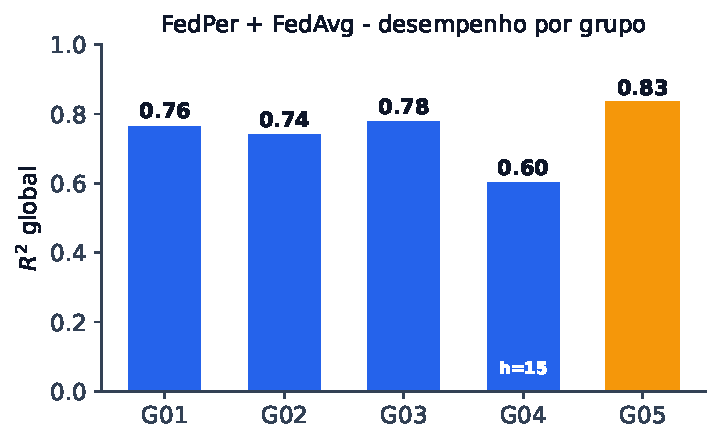
\includegraphics[width=\linewidth]{figures/results_r2.pdf}
    \end{column}
    \begin{column}{0.42\textwidth}
      \small
      O melhor modelo (\textbf{FedPer + FedAvg}) foi avaliado em todos os grupos:
      \begin{itemize}
        \item $R^2$ entre \textbf{0,60} e \textbf{0,83}.
        \item Melhor em \textbf{G05} (ICE 2.0L): $0{,}83$.
        \item \textbf{G04} previu um horizonte maior (15 passos), tarefa mais
              difícil: $0{,}60$.
      \end{itemize}
      Em todos, a cauda local capturou o comportamento de cada veículo.
    \end{column}
  \end{columns}
  \vspace{2pt}
\end{frame}

\begin{frame}{Como o erro cresce com o horizonte}
  \begin{columns}[T]
    \begin{column}{0.56\textwidth}
      \centering
      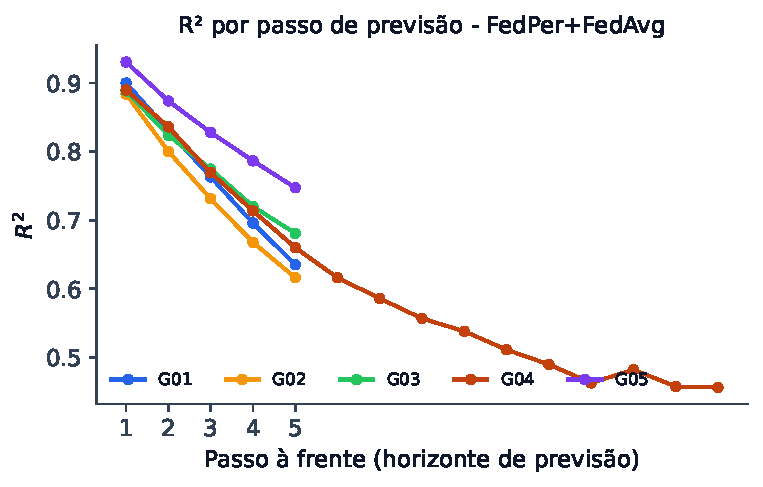
\includegraphics[width=\linewidth]{figures/results_r2_step.pdf}
    \end{column}
    \begin{column}{0.44\textwidth}
      \small
      O modelo prevê vários \textbf{passos à frente} de uma vez. O passo~1 é a
      leitura logo em seguida; os seguintes são cada vez mais distantes no futuro.
      \medskip

      Quanto mais longe, mais difícil: o $R^2$ \textbf{cai} a cada passo.
      \begin{itemize}
        \item Passo~1: $R^2 \approx 0{,}9$ em todos os grupos.
        \item O G04 vai até o passo~15, mostrando a degradação num horizonte
              bem mais longo.
      \end{itemize}
    \end{column}
  \end{columns}
  \vspace{2pt}
\end{frame}

% =====================================================================
\section{Conclusão}

\begin{frame}{Em resumo}
  \begin{itemize}
    \item O Fleven treina modelos de consumo sem centralizar dados dos veículos.
    \item A agregação combina os modelos locais; \textbf{FedAvg} foi a mais estável.
    \item \textbf{FedPer} personaliza por veículo e teve o melhor desempenho no eVED.
  \end{itemize}
\end{frame}

\begin{frame}[allowframebreaks]{Referências}
  \footnotesize
  \bibliographystyle{apalike}
  \bibliography{ref}
\end{frame}

\end{document}